
Design Science Research in information systems is a methodology for creating new knowledge by designing, building and evaluating software \glspl{artifact}.
It may not be as widely known as ``the scientific method'' is, and is therefore explained in more detail.

\paragraph{Design}
\textit{Design} in information systems is an iterative process and a resulting software artifact. A software artifact is to be built to solve problems for humans, and evaluated to prove it solves the problems~\cite[p.~2]{alanhevnerDesignResearchInformation2010}.


\paragraph{Research}
\textit{Research} is an activity that adds new knowledge and understanding about something.
Research should be systematical and use data to answer questions, solve problems and provide understanding~\cite[p.~2,3]{alanhevnerDesignResearchInformation2010}.

\paragraph{Design Science Research}
\textit{Design Science Research} is an approach to research where knowledge is created by design.
It is defined by \textcite[p.~5]{alanhevnerDesignResearchInformation2010} as follows:

\begin{quote}
  \textit{``Design science research is a research paradigm in which a designer answers questions relevant to human problems via the creation of innovative artifacts, thereby contributing new knowledge to the body of scientific evidence.
  The designed artifacts are both useful and fundamental in understanding that problem.''}
\end{quote}

The end goal of a Design Science Research project is to create information technology \glspl{artifact}, that improve exiting solutions or solve a problem for the first time~\cite[p.~6]{alanhevnerDesignResearchInformation2010}.
A similar methodology may also be known under the name \textit{Design and Creation}, as presented by \textcite[p.~108]{oatesResearchingInformationSystems2006}.
According to \textcite{alanhevnerDesignResearchInformation2010}, the artifacts are generally classified as \textit{constructs}, \textit{models}, \textit{methods}, \textit{instantiations} or \textit{better design theories}%
\label{par:artifact-classes}%
\footnote{This thesis aims to produce an instantiation: an implemented or prototype system. The thesis also seeks to advance on \textit{better design theories}, with regards to software architecture and protocol design.}.
A very important aspect of Design Science Research is \textit{evaluation} of the artifact.
The evaluation is the process that uncovers new knowledge, and separates the process from routine design~\cite[p.~7]{alanhevnerDesignResearchInformation2010}.
There are many aspects that could be evaluated, but the aspects that \textit{should} be evaluated are those that are related to the reason for creating the artifact in the first place; the aspects related to the research objectives~\cite[p.~115]{oatesResearchingInformationSystems2006}.


% TODO

\subsection{The General Design Cycle }

\paragraph{Design Cycle}
Problem solving by design can follow a general design cycle.
This is a circular and iterative process.
The reasoning that occurs in a design cycle, and the knowledge generated during a cycle, is illustrated in \cref{fig:dsrpm}~\cite[p.~26]{alanhevnerDesignResearchInformation2010}.

\begin{figure}[htbp]  % order of priority: h here, t top, b bottom, p page
  \centering
  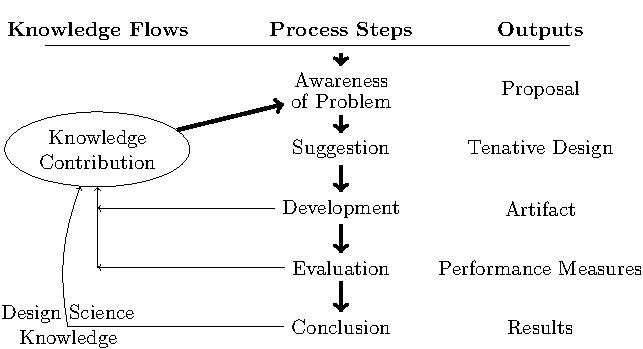
\includegraphics[width=\textwidth]{figures/dsrm-flow.pdf}
  \caption[Design Science Research Process Model]{\textbf{Design Science Research Process Model}. The general process followed by Design Science Research. Design begins with awareness of a problem, and progresses through a suggestion for a solution, to development, evaluation and a conclusion.
  The stages produce different outputs, shown in the right column.
  After the conclusion, new knowledge is contributed.
  There is also knowledge produced by development and evaluation, nicknamed ``circumscription''.
  This knowledge is fed back into a new round of suggestion~\cite[p.~11-13]{vijayvaishnaviDesignScienceResearch2019}.
  (Adopted from Figure 3 in \textcite[p.~11]{vijayvaishnaviDesignScienceResearch2019})}\label{fig:dsrpm}
\end{figure}


\paragraph{Awareness of Problem}
The process begins by becoming aware of a problem or opportunities, in the context of humans or an organization.
A proposal for what could be solved is made explicit.


\paragraph{Suggestion}
Then, a suggestion phase begins, where existing knowledge and theories are applied, as well as creativity, to create a tentative design that fits the proposal.
This design could be flawed or incorrect, which is why it is important to realize the design, to detect issues.


\paragraph{Development}
The development phase will build a solution or prototype, aiming to fulfill the suggested design.
This phase will uncover problems, inconsistencies, new learning about the problem, and other related knowledge.
That knowledge is useful for creating a new and improved design.
The quality of the \textit{implementation} of the artifact does not need to be novel, as it is the \textit{design} which is interesting~\cite[p.~12]{vijayvaishnaviDesignScienceResearch2019}.


\paragraph{Evaluation}
After an artifact is created, the evaluation phase will measure the artifact.
The measurements originate from the initial proposal, which holds the criteria for success.
This phase may also discover new knowledge, which can be used later to create a new and improved design~\cite[p.~13]{vijayvaishnaviDesignScienceResearch2019}.


\paragraph{Conclusion}
Finally, the conclusion phase will consolidate the results.
The knowledge gained from the results will either be ``firm'' or ``loose ends''.
\Textcite[p.~13]{vijayvaishnaviDesignScienceResearch2019} describes this as the following:

\begin{quote}
``\textit{Not only are the results of the effort consolidated and ``written up'' at this phase, but the knowledge gained in the effort is frequently categorized as either ``firm'' --- facts that have been learned and can be repeatedly applied or behavior that can be repeatedly invoked --- or as ``loose ends'' --- anomalous behavior that defies explanation and may well serve as the subject of further research.}''
\end{quote}


\subsection{Methodology}

Based on the understanding of design science research, and the steps of a design science research process (\cref{fig:dsrpm}), a six step Design Science Research Methodology has been made by \textcite[p.~28-30]{alanhevnerDesignResearchInformation2010}.
This methodology forms the skeleton of this thesis.
The six steps of the methodology are the following:

\begin{enumerate}
  \item \textit{Problem identification and motivation.}
  \item \textit{Define the objectives for a solution.}
  \item \textit{Design and development.}
  \item \textit{Demonstration.}
  \item \textit{Evaluation.}
  \item \textit{Communication.}
\end{enumerate}


\paragraph{1. Problem identification and motivation}
The specific research problem must be defined.
The definition is used to develop the artifact which solves the problem.
The value of a solution to the problem should be justified as well.
If the value of the solution is justified, it can motivate the researcher and the thesis' audience to pursue the solution and accept the results~\cite[p.~28,29]{alanhevnerDesignResearchInformation2010}.

\paragraph{2. Define the objectives for a solution}
The objectives should be inferred from the problem definition, and the author's knowledge of what is possible and feasible.
The objectives can be how much better a new solution should be (quantitative), or a description of how a new artifact would solve problems that are currently unsolved (qualitative)~\cite[p.~29]{alanhevnerDesignResearchInformation2010}.

\paragraph{3. Design and development}
Create an artifact to solve the problem and fulfill the objectives.
The artifact can be one of the five classes listed in \cref{par:artifact-classes} (constructs, models etc.).
The desired functionality and architecture is determined, and the actual artifact is created~\cite[p.~29]{alanhevnerDesignResearchInformation2010}.


\paragraph{4. Demonstration}
The artifact is demonstrated, to solve instances of the identified problem.
This could be experiments, simulations, case studies etc.~\cite[p.~30]{alanhevnerDesignResearchInformation2010}.


\paragraph{5. Evaluation}
The artifact is observed and evaluated to measure how well it solves the identified problem.
This can be done by comparing the results of the demonstration to the  objectives of an ideal solution.
There are many different ways to evaluate an artifact, and the correct approach should be decided based on the nature of the identified problem.
After evaluation, the researcher can go back to step 3 to improve the design.
If there is not enough time, resources or a need to do so, the process moves to step 6 instead~\cite[p.~30]{alanhevnerDesignResearchInformation2010}.

\paragraph{6. Communication}
The process must be communicated to other researchers and relevant audiences.
This communication includes: the problem and its importance, the artifact and its utility, the rigor of the artifact design, and the effectiveness of the design~\cite[p.~30]{alanhevnerDesignResearchInformation2010}.%
\footnote{This thesis is a central part of this communication.}

